\chapter{Background}
\label{chap:background}

\section{Dust Modeling}

Interstellar dust plays a fundamental role in tracing the structure of molecular clouds (CITATION). Though it accounts for only about 1\% of the mass of the interstellar medium (ISM), its ability to absorb, scatter, and re-emit radiation makes it an essential tool for indirectly probing the properties of cold, dense gas where stars form.

\subsection{Emission from Dust Grains}

Dust grains absorb ultraviolet (UV), visible, and near-infrared (NIR) radiation from stars and re-emit this energy thermally at longer wavelengths, primarily in the mid-infrared (MIR), far-infrared (FIR), and submillimeter (sub-mm) regimes. This process is governed by the radiative transfer equation, which couples extinction (absorption and scattering) and emission across the electromagnetic spectrum (CITATION). In molecular clouds, where visual extinction can exceed $A_V > 10$, emission from dust becomes the dominant observable at long wavelengths.

Dust emission is commonly modeled as a modified black-body, or "grey-body," spectrum:
\[
F_\nu^{\mathrm{obs}} = B_\nu(T_\mathrm{dust}) \times \left(1 - e^{-\tau_\nu}\right),
\]
where $B_\nu(T_\mathrm{dust})$ is the Planck function at the dust temperature $T_\mathrm{dust}$, and $\tau_\nu$ is the optical depth at frequency $\nu$. For optically thin emission at long wavelengths ($\tau_\nu \ll 1$), this simplifies to:
\[
F_\nu^{\mathrm{obs}} \approx B_\nu(T_\mathrm{dust}) \cdot \tau_\nu.
\]

The optical depth $\tau_\nu$ is typically parameterized as:
\[
\tau_\nu = \kappa_\nu \cdot \Sigma,
\]
where $\kappa_\nu$ is the dust opacity and $\Sigma$ the dust surface density. The dust opacity is often modeled as a power-law:
\[
\kappa_\nu \propto \nu^\beta,
\]
where $\beta$ is the dust emissivity index, typically between 1.5 and 2 in the ISM.

\subsection{Rayleigh–Jeans Approximation and FIR Observations}

To reduce the number of free parameters when inferring dust properties, observations are often carried out in the Rayleigh–Jeans (RJ) regime, where $h\nu \ll k_B T$. This condition is typically satisfied at wavelengths longer than $\sim 250\,\mu$m for dust temperatures around $T_\mathrm{dust} \sim 10$–$20$ K, which makes submillimeter and millimeter observations (e.g. from \textit{Herschel}) particularly valuable.

In this regime, the flux scales as:
\[
F_\nu^{\mathrm{obs}} \propto \nu^{2+\beta},
\]
allowing for simplified spectral energy distribution (SED) fitting to extract the dust temperature and column density.

\subsection{Column Density Estimation}

Under the assumption of fixed dust opacity $\kappa_{850}$ and emissivity index $\beta$, one can solve for the dust optical depth at a reference frequency (e.g., $850\,\mu$m):
\[
\tau_{850} = \frac{I_{850}}{B_{850}(T_\mathrm{dust})}.
\]
Given a calibration between optical depth and column density (e.g., from \cite{hildebrand1983determination}), the molecular hydrogen column density $N(\mathrm{H}_2)$ can be in principle estimated as:
\[
N(\mathrm{H}_2) \propto \tau_{850}.
\]

This method allows for the derivation of full-resolution column density maps from multi-band FIR/sub-mm observations, as performed by the \textit{Herschel} Gould Belt Survey, providing a key data product for structural and fractal analyses.

\subsection{Comparison with Extinction Methods}

\begin{figure}[t]
    \centering
    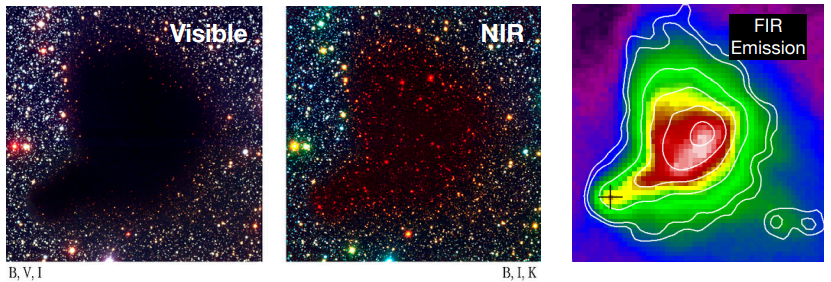
\includegraphics[width=0.75\textwidth]{figures/comparison_dust.png}
    \caption{Comparison of dust extinction (optical and NIR) and dust emission (FIR) views of Barnard 68. Credits: ESO, \cite{nielbock2012earliest}.}
    \label{fig:comparison_dust}
\end{figure}

Dust column densities can also be inferred from extinction measurements, particularly in the near-infrared (e.g., via NICER/NICEST , CITATION). These techniques are independent of dust temperature and often provide high angular resolution in regions with abundant background stars. However, their reliability decreases in high-opacity areas, where few background stars are detectable, and they require robust modeling of the stellar background.

Emission-based methods, by contrast, are more effective in probing dense and cold regions. By modeling the thermal emission from dust at far-infrared and sub-millimeter wavelengths, they can recover column density even where extinction saturates. Nevertheless, these methods rely on assumptions about dust temperature, opacity laws, and emissivity index, which can introduce systematic uncertainties.

Each approach has its strengths and limitations, and the choice between them depends on the scientific objectives and the characteristics of the target region. A visual comparison of both techniques is shown in Figure~\ref{fig:comparison_dust}, highlighting the complementary nature of extinction and emission observations for the dark cloud Barnard 68.

\subsection{Relevance to Star Formation}

Dust-based column density maps are crucial for studying the early stages of star formation. Since most dust in molecular clouds is cold ($T_\mathrm{dust} \sim 10{-}20\,\mathrm{K}$), emission in the FIR/sub-mm naturally traces the dense gas where star formation occurs. Thresholds in column density (e.g., $N(\mathrm{H}_2) \sim 1{-}2 \times 10^{22}\,\mathrm{cm}^{-2}$) have been associated with the onset of core formation and gravitational instability \cite{lada2010star}.

Thus, dust modeling serves as the foundation for the structural and statistical analyses performed throughout this thesis.

\section{Fractals}

Fractals are geometric objects characterized by irregularity and self-similarity over a range of scales. Unlike classical Euclidean shapes, fractals cannot be described by integer dimensions and often exhibit complex, nested structures. Introduced to the scientific community largely through the work of Mandelbrot in the late 20th century (CITATION), fractal geometry has since become a powerful framework for describing naturally occurring structures, from coastlines to clouds.

In the context of molecular clouds, fractal behavior arises seemingly naturally everywhere we look. These regions of the interstellar medium exhibit turbulent dynamics and hierarchical fragmentation, producing morphologies that lack a characteristic scale. Theoretical models of interstellar turbulence, particularly those based on compressible, supersonic flows, predict self-similar density structures (CITATION). Observational studies have consistently found evidence of such fractal-like properties in molecular clouds, supporting the idea that turbulence plays a dominant role in shaping them \cite{elmegreen1996fractal, falgarone1991hierarchical}.

The \emph{fractal dimension} is a key quantitative descriptor of a structure's complexity.  Unlike topological dimension, the fractal dimension can take non-integer values and is sensitive to the method used to estimate it. In this work, we explore this quantity through the perimeter–area relation and other related approaches, which are introduced in detail in later chapters.

Understanding fractal properties is not just a matter of geometry. The morphology of molecular clouds is intimately connected to their physical evolution. For instance, more fragmented structures may reflect advanced stages of gravitational collapse or be the signature of driven turbulence. Moreover, star formation tends to occur in regions of low complexity and high density, suggesting a link between the fractal nature of clouds and their star-forming potential.

In summary, fractal geometry offers an intuitive and quantitative framework to describe the hierarchical, scale-free nature of molecular clouds. Combined with other morphological and topological tools, it provides valuable insights into the processes that govern the interstellar medium and the onset of star formation. Combining these techniques with dust emission maps will allow us to quantitatively characterize the structure of molecular clouds across a wide range of spatial scales. This integrated approach enables the identification of correlations between cloud morphology, physical conditions, and star formation activity, thereby advancing our understanding of the complex interplay between turbulence, gravity, and feedback in the interstellar medium.